\documentclass{scrreprt}

\usepackage{aligned-overset}
\usepackage{amsmath}
\usepackage{amssymb}
\usepackage{bm}
\usepackage[shortlabels]{enumitem}
\usepackage{hyperref}
\usepackage[utf8]{inputenc}
\usepackage{multicol}
\usepackage{mathtools}
\usepackage{physics}
\usepackage{tabularx}
\usepackage{titling}
\usepackage{fancyhdr}
\usepackage{xfrac}
\usepackage{pgfplots}

\pgfplotsset{compat = newest}
\usetikzlibrary{intersections}
\usetikzlibrary{patterns}
\usetikzlibrary{positioning}
\usetikzlibrary{shapes.misc}
\usepgfplotslibrary{fillbetween}

\author{Karsten Lehmann}
\date{WiSe 2021/2022}
\title{Übungsblatt 02\\Algorithmen und Datenstrukturen}

\setlength{\headheight}{26pt}
\pagestyle{fancy}
\fancyhf{}
\lhead{\thetitle}
\rhead{\theauthor}
\lfoot{\thedate}
\rfoot{Seite \thepage}

\begin{document}
\paragraph{Aufgabe 1} Das folgende Syntaxdiagrammsystem $\mathcal{U}$ ist
gegeben, $S$ ist das Startdiagramm: \\
\begin{tikzpicture}
  \node at (0, 0) {S};
  \node[circle, draw] (a) at (1, -1) {a};
  \node[draw, right = of a, rectangle] (B) {B};
  \node[fill = yellow, above right = 0 of B] {{\tiny $S_1$}};
  \node[below = 0.5 of B, circle, draw] (c1) {c};
  \node[circle, draw, right = 0.5 of c1] (c2) {c};
  \node[circle, draw, right = 2 of B] (b) {b};
  \draw (a) -- ++(-1, 0);
  \draw (a) -- (B);
  \draw (B) -- (b);
  \draw (b) -- ++(1, 0);
  \draw (c1) -- (c2);
  \draw (c1) .. controls ++(-0.8,0) and ++(0.4,0) .. ++(-.8, 1.05);
  \draw (c2) .. controls ++(0.8,0) and ++(-0.4,0) .. ++(.8, 1.05);
\end{tikzpicture}
\begin{tikzpicture}
  \node at (0, 0) {B};
  \node[circle, draw] (a) at (2, -1) {a};
  \node[draw, right = 0.5 of a, rectangle] (B) {B};
  \node[fill = yellow, above right = 0 of B] {{\tiny $B_1$}};
  \node[right = 0.6 of B, circle, draw] (d) {d};
  \node[below = 0.5 of a, draw, rectangle] (S) {S};
  \node[fill = yellow, above right = 0 of S] {{\tiny $B_2$}};
  \draw (a) -- ++(-2, 0);
  \draw (a) -- (B);
  \draw (B) -- (d);
  \draw (d) -- ++(2, 0);
  \draw (S) .. controls ++(-0.8,0) and ++(0.4,0) .. ++(-.8, 1.05);
  \draw (S) -- ++(2.5, 0) .. controls ++(0.8,0) and ++(-0.4,0) .. ++(.8, 1.05);
\end{tikzpicture}
\begin{enumerate}[(a)]
\item Geben Sie zwei Wörter in der Sprache von $\mathcal{U}$ an, die länger als
  4 Zeichen sind.
  Nutzen Sie dafür den Rücksprungalgorithmus.
  Wie stehen die Vorkommen von \textbf{a} zu den Vorkommen von \textbf{b} und
  \textbf{d} in der Wörtern der Sprache von $\mathcal{U}$ im Verhältnis?

  \subparagraph{Lsg.} Wörter in der Sprache von $\mathcal{U}$, die länger als
  4 Zeichen sind umfassen zum Beispiel \emph{aaccbb}, \emph{aaaccbdb} und
  \emph{aaaaccbddb}.

  Das \emph{c} kommt dabei in jedem Wort genau zweimal vor.
  Es ist notwendig den Pfad mit den beiden \emph{c}'s zu durchlaufen, um zum
  Ende des Syntaxdiagrammes zu kommen und gleichzeitig kann dieser Pfad nur ein
  einziges Mal durchlaufen werden.

  Die Menge der Vorkommen der \emph{b}'s und \emph{d}'s addiert ergibt die Menge
  der \emph{a}'s.

\item Zeigen sie mit Hilfe des Rücksprungalgorihmus, dass das Wort
  \textbf{aaaaccbdbb} zu der durch $\mathcal{U}$ definierten Sprache gehört.
  Fertigen Sie ein entsprechendes Markenprotokoll an.

  \subparagraph{Lsg.} in dem gegebenen Syntaxdiagrammsystem $\mathcal{U}$ gibt
  es genau 2 Stellen an welche zurückgesprungen werden kann.
  Diese Stellen sind \colorbox{yellow}{farbig} mit $S_1$, $B_1$ und $B_2$
  markiert.

  \begin{small}
  \begin{tabularx}{\linewidth}{X|c|c}
    \textbf{Schritt} & \textbf{Wort} & \textbf{Keller} \\
    \hline
    1. Beginne am Eingang des Startdiagramms - in diesem Fall des
    Syntaxdiagramms ``S''. & & \\
    2. Folge den Linien auf einem legalen Weg - hier zum Oval \textbf{a} - und
    gehe zu Punkt 3 & & \\
    3. Falls es sich um ein Oval handelt, notiere das darin enthaltene
    Terminalzeichen und gehe zu Punkt 2 zurück. & \emph{a} & \\
    2. Folge den Linien auf einem legalen Weg - hier zum Kästchen \textbf{B} -
    und gehe zu Punkt 3 & \emph{a} & \\
    3. Falls es sich um ein Kästchen handelt gehe zu Punkt 4 & \emph{a} & \\
    4. Lege eine Kopie der Rücksprungadresse - hier $S_1$ - oben auf den Keller,
    suche den Eingang des neuen Diagramms und arbeite ab Punkt 2 weiter. &
    \emph{a} & $S_1$ \\
    2. Folge den Linien auf einem legalen Weg - hier zum Kästchen \textbf{S} -
    und gehe zu Punkt 3 & \emph{a} & $S_1$ \\
    3. Falls es sich um ein Kästchen handelt gehe zu Punkt 4 & \emph{a} &
    $S_1$ \\
  \end{tabularx}
  \end{small}

  \begin{small}
  \begin{tabularx}{\linewidth}{X|c|c}
    \textbf{Schritt} & \textbf{Wort} & \textbf{Keller} \\
    \hline
    4. Lege eine Kopie der Rücksprungadresse - hier $B_2$ - oben auf den Keller,
    suche den Eingang des neuen Diagramms und arbeite ab Punkt 2 weiter. &
    \emph{a} & $S_1, B_2$ \\
    2. Folge den Linien auf einem legalen Weg - hier zum Oval \textbf{a} - und
    gehe zu Punkt 3 & \emph{a} & $S_1, B_2$ \\
    3. Falls es sich um ein Oval handelt, notiere das darin enthaltene
    Terminalzeichen und gehe zu Punkt 2 zurück. & \emph{aa} & $S_1, B_2$ \\
    2. Folge den Linien auf einem legalen Weg - hier zum Kästchen \textbf{B} -
    und gehe zu Punkt 3 & \emph{aa} & $S_1, B_2$ \\
    3. Falls es sich um ein Kästchen handelt gehe zu Punkt 4  & \emph{aa} &
    $S_1, B_2$ \\
    4. Lege eine Kopie der Rücksprungadresse - hier $S_1$ - oben auf den Keller,
    suche den Eingang des neuen Diagramms und arbeite ab Punkt 2 weiter. &
    \emph{aa} & $S_1, B_2, S_1$ \\
    2. Folge den Linien auf einem legalen Weg - hier zum Oval \textbf{a} - und
    gehe zu Punkt 3 & \emph{aa} & $S_1, B_2, S_1$ \\
    3. Falls es sich um ein Oval handelt, notiere das darin enthaltene
    Terminalzeichen und gehe zu Punkt 2 zurück.
    & \emph{aaa} & $S_1, B_2, S_1$ \\
    2. Folge den Linien auf einem legalen Weg - hier zum Kästchen \textbf{B} -
    und gehe zu Punkt 3 & \emph{aaa} & $S_1, B_2, S_1$ \\
    3. Falls es sich um ein Kästchen handelt gehe zu Punkt 4
    & \emph{aaa} & $S_1, B_2, S_1$ \\
    4. Lege eine Kopie der Rücksprungadresse - hier $B_1$ - oben auf den Keller,
    suche den Eingang des neuen Diagramms und arbeite ab Punkt 2 weiter.
    & \emph{aaa} & $S_1, B_2, S_1, B_1$ \\
    2. Folge den Linien auf einem legalen Weg - hier zum Kästchen \textbf{S} -
    und gehe zu Punkt 3 & \emph{aaa} & $S_1, B_2, S_1, B_1$ \\
    3. Falls es sich um ein Kästchen handelt gehe zu Punkt 4
    & \emph{aaa} & $S_1, B_2, S_1, B_1$ \\
    4. Lege eine Kopie der Rücksprungadresse - hier $B_2$ - oben auf den Keller,
    suche den Eingang des neuen Diagramms und arbeite ab Punkt 2 weiter.
    & \emph{aaa} & $S_1, B_2, S_1, B_1, B_2$ \\
    2. Folge den Linien auf einem legalen Weg - hier zum Oval \textbf{a} - und
    gehe zu Punkt 3 & \emph{aaa} & $S_1, B_2, S_1, B_1, B_2$ \\
    3. Falls es sich um ein Oval handelt, notiere das darin enthaltene
    Terminalzeichen und gehe zu Punkt 2 zurück.
    & \emph{aaaa} & $S_1, B_2, S_1, B_1, B_2$ \\
    2. Folge den Linien auf einem legalen Weg - hier zum Oval \textbf{c} - und
    gehe zu Punkt 3 & \emph{aaaa} & $S_1, B_2, S_1, B_1, B_2$ \\
    3. Falls es sich um ein Oval handelt, notiere das darin enthaltene
    Terminalzeichen und gehe zu Punkt 2 zurück.
    & \emph{aaaac} & $S_1, B_2, S_1, B_1, B_2$ \\
    2. Folge den Linien auf einem legalen Weg - hier zum Oval \textbf{c} - und
    gehe zu Punkt 3 & \emph{aaaac} & $S_1, B_2, S_1, B_1, B_2$ \\
    3. Falls es sich um ein Oval handelt, notiere das darin enthaltene
    Terminalzeichen und gehe zu Punkt 2 zurück.
    & \emph{aaaacc} & $S_1, B_2, S_1, B_1, B_2$ \\
    2. Folge den Linien auf einem legalen Weg - hier zum Oval \textbf{b} - und
    gehe zu Punkt 3 & \emph{aaaacc} & $S_1, B_2, S_1, B_1, B_2$ \\
    3. Falls es sich um ein Oval handelt, notiere das darin enthaltene
    Terminalzeichen und gehe zu Punkt 2 zurück.
    & \emph{aaaaccb} & $S_1, B_2, S_1, B_1, B_2$ \\
    2. Folge den Linien auf einem legalen Weg - hier zum Ausgang - und
    gehe zu Punkt 5 & \emph{aaaaccb} & $S_1, B_2, S_1, B_1, B_2$ \\
  \end{tabularx}
  \end{small}

  \begin{small}
  \begin{tabularx}{\linewidth}{X|c|c}
    \textbf{Schritt} & \textbf{Wort} & \textbf{Keller} \\
    \hline
    5. Wenn eine Rücksprungadresse auf dem Keller liegt, dann nimm diese
    herunter und fahre an der Adresse mit Punkt 2 fort.
    & \emph{aaaaccb} & $S_1, B_2, S_1, B_1$ \\
    2. Folge den Linien auf einem legalen Weg - hier zum Ausgang - und
    gehe zu Punkt 5 & \emph{aaaaccb} & $S_1, B_2, S_1, B_1$ \\
    5. Wenn eine Rücksprungadresse auf dem Keller liegt, dann nimm diese
    herunter und fahre an der Adresse mit Punkt 2 fort.
    & \emph{aaaaccb} & $S_1, B_2, S_1$ \\
    2. Folge den Linien auf einem legalen Weg - hier zum Oval \textbf{d} - und
    gehe zu Punkt 3 & \emph{aaaaccb} & $S_1, B_2, S_1$ \\
    3. Falls es sich um ein Oval handelt, notiere das darin enthaltene
    Terminalzeichen und gehe zu Punkt 2 zurück.
    & \emph{aaaaccbd} & $S_1, B_2, S_1$ \\
    2. Folge den Linien auf einem legalen Weg - hier zum Ausgang - und
    gehe zu Punkt 5 & \emph{aaaaccbd} & $S_1, B_2, S_1$ \\
    5. Wenn eine Rücksprungadresse auf dem Keller liegt, dann nimm diese
    herunter und fahre an der Adresse mit Punkt 2 fort.
    & \emph{aaaaccbd} & $S_1, B_2$ \\
    2. Folge den Linien auf einem legalen Weg - hier zum Oval \textbf{b} - und
    gehe zu Punkt 3 & \emph{aaaaccbd} & $S_1, B_2$ \\
    3. Falls es sich um ein Oval handelt, notiere das darin enthaltene
    Terminalzeichen und gehe zu Punkt 2 zurück.
    & \emph{aaaaccbdb} & $S_1, B_2$ \\
    2. Folge den Linien auf einem legalen Weg - hier zum Ausgang - und
    gehe zu Punkt 5 & \emph{aaaaccbdb} & $S_1, B_2$ \\
    5. Wenn eine Rücksprungadresse auf dem Keller liegt, dann nimm diese
    herunter und fahre an der Adresse mit Punkt 2 fort.
    & \emph{aaaaccbdb} & $S_1$ \\
    2. Folge den Linien auf einem legalen Weg - hier zum Ausgang - und
    gehe zu Punkt 5 & \emph{aaaaccbdb} & $S_1$ \\
    5. Wenn eine Rücksprungadresse auf dem Keller liegt, dann nimm diese
    herunter und fahre an der Adresse mit Punkt 2 fort.
    & \emph{aaaaccbdb} & \\
    2. Folge den Linien auf einem legalen Weg - hier zum Oval \textbf{b} - und
    gehe zu Punkt 3 & \emph{aaaaccbdb} & \\
    3. Falls es sich um ein Oval handelt, notiere das darin enthaltene
    Terminalzeichen und gehe zu Punkt 2 zurück.
    & \emph{aaaaccbdbb} & \\
    2. Folge den Linien auf einem legalen Weg - hier zum Ausgang - und
    gehe zu Punkt 5 & \emph{aaaaccbdbb} & \\
    5. Wenn keine Rücksprungadresse auf dem Keller liegt ist der Prozess zu Ende
    & \emph{aaaaccbdbb} & \\
  \end{tabularx}
  \end{small}

\newpage
\item Gegeben Sei die folgende Sprache
  $L = \qty\big{a^{2i}cb^{3i}c^kd^{2k + 1} \,{\big |}\, i > 0, k \geq 0}$.
  Geben Sie für $L$ ein System von Syntaxdiagrammen an, welches genau diese
  Sprache erzeugt.

  \subparagraph{Lsg.} Die Sprache wird von dem folgenden System von
  Syntaxdiagrammen mit dem Startdiagramm \emph{A} erzeugt: \\
  \begin{tikzpicture}
    \node at (0, 0) {A};
    \node[draw, rectangle] (B) at (1, -1) {B};
    \node[draw, rectangle, right = of B] (C) {C};
    \node[circle, draw, right = of C] (d) {d};
    \draw (B) -- ++(-1, 0);
    \draw (B) -- (C);
    \draw (C) -- (d);
    \draw (d) -- ++(1, 0);
  \end{tikzpicture}

  \begin{tikzpicture}
    \node at (0, 0) {B};
    \node[circle, draw] (a1) at (1, -1) {a};
    \node[circle, draw, right = 0.5 of a1] (a2) {a};
    \node[draw, rectangle, right = of a2] (B) {B};
    \node[circle, draw, right = of B] (b1) {b};
    \node[circle, draw, right = 0.5 of b1] (b2) {b};
    \node[circle, draw, right = 0.5 of b2] (b3) {b};
    \node[below = 0.5 of B, circle, draw] (c) {c};
    \draw (a1) -- ++(-1, 0);
    \draw (a1) -- (a2);
    \draw (a2) -- (B);
    \draw (B) -- (b1);
    \draw (b1) -- (b2);
    \draw (b2) -- (b3);
    \draw (b3) -- ++(1, 0);
    \draw (c) .. controls ++(-0.8,0) and ++(0.4,0) .. ++(-.8, 1.05);
    \draw (c) .. controls ++(0.8,0) and ++(-0.4,0) .. ++(.8, 1.05);
  \end{tikzpicture}

  \begin{tikzpicture}
    \node at (0, 0) {C};
    \node[circle, draw] (c) at (2, -1) {c};
    \node[draw, rectangle, right = 0.5 of c] (C) {C};
    \node[circle, draw, right = 0.5 of C] (d1) {d};
    \node[circle, draw, right = 0.5 of d1] (d2) {d};
    \draw (0, -1) -- (c) -- (C) -- (d1) -- (d2) -- ++(2, 0);
    \draw (1, -1) .. controls ++(0.4,0) and ++(-0.8,0) .. ++(.8, -1.05)
      -- ++(4, 0) .. controls ++(0.8,0) and ++(-0.4,0) .. ++(.8, 1.05);
  \end{tikzpicture}
\end{enumerate}

\paragraph{Aufgabe 2} Gegeben Sei die EBNF-Definition
$\varepsilon = \qty\big(V, \Sigma, A, R)$ mit $V = \qty\big{A, B, C}$,
$\Sigma = \qty\big{a, b, c, d}$ und
\[
  R = \qty\big{
    A \Coloneqq BC,
    B \Coloneqq \hat{(}aBc \,\hat{|}\, \hat{\{}b\hat{\}}\hat{)},
    C \Coloneqq d \hat{[} C \hat{]} c
  }
\]
\begin{enumerate}[(a)]
\item Übersetzen Sie $\varepsilon$ gemäß der Übersetzungsvorschrift \emph{trans}
  aus der Vorlesung in ein System von Syntaxdiagrammen und geben Sie das
  Startdiagramm an.

  \subparagraph{Lsg.} Das Startdiagramm ist \emph{A}: \\
  \begin{tikzpicture}
    \node at (0, 0) {A};
    \node[draw, rounded rectangle] (A1) at (2, -1) {$\emph{trans}(BC)$};
    \draw (0, -1) -- (A1) -- ++(2, 0);
    \node[draw, rounded rectangle] (A2_1) at (2, -2) {$\emph{trans}(B)$};
    \node[draw, rounded rectangle] (A2_2) at (4, -2) {$\emph{trans}(C)$};
    \draw (0, -2) -- (A2_1) -- (A2_2) -- ++(2, 0);
    \node[draw, rectangle] (A3_1) at (1, -3) {B};
    \node[draw, rectangle, right = 0.5 of A3_1] (A3_2) {C};
    \draw (0, -3) -- (A3_1) -- (A3_2) -- ++(1, 0);
  \end{tikzpicture}

  \begin{tikzpicture}
    \node at (0, 0) {B};
    \node[draw, rounded rectangle] (B1) at (2, -1) {$\emph{trans}(\hat{(}aBc \,\hat{|}\, \hat{\{}b\hat{\}}\hat{)})$};
    \draw (0, -1) -- (B1) -- ++(2, 0);

    \node[draw, rounded rectangle] (B2_1) at (2.5, -2) {$\emph{trans}(aBc)$};
    \node[draw, rounded rectangle] (B2_2) at (2.5, -3) {$\emph{trans}(\hat{\{}b\hat{\}})$};
    \draw (0, -2) -- (B2_1) -- ++(2.5, 0);
    \draw (0.75, -2) .. controls ++(0.5,0) and ++(-1.8,0) .. (B2_2)
      .. controls ++(1.8,0) and ++(-0.5,0) .. ++(1.8, 1);

    \node[draw, rounded rectangle] (B3_1) at (2.5, -4) {$\emph{trans}(a)$};
    \node[draw, right = 0.5 of B3_1, rounded rectangle] (B3_2) {$\emph{trans}(B)$};
    \node[draw, right = 0.5 of B3_2, rounded rectangle] (B3_3) {$\emph{trans}(c)$};
    \node[below = 1.35 of B3_2, draw, rounded rectangle] (B3_4) {$\emph{trans}(b)$};
    \draw (0, -4) -- (B3_1) -- (B3_2) -- (B3_3) -- ++(2.5, 0);
    \draw (0.75, -4) .. controls ++(0.8,0) and ++(-0.8,0) .. ++(0.8, -1) -- ++(6.5, 0)
      .. controls ++(0.8,0) and ++(-0.8,0) .. ++(0.8, 1);
    \draw (3.5, -5) .. controls ++(-0.4,0) and ++(0,0.4) .. ++(-0.5, -0.5)
      .. controls ++(0, -0.4) and ++(-0.4, 0) .. ++(+0.5, -0.5) -- (B3_4);
    \draw (6, -5) .. controls ++(0.4,0) and ++(0,0.4) .. ++(0.5, -0.5)
      .. controls ++(0, -0.4) and ++(0.4, 0) .. ++(-0.5, -0.5) -- (B3_4);

    \node[circle, draw] (B4_1) at (1.5, -7) {a};
    \node[draw, right = 0.5 of B4_1, rectangle] (B4_2) {B};
    \node[circle, draw, right = 0.5 of B4_2] (B4_3) {c};
    \node[below = 0.8 of B4_2, circle, draw] (B4_4) {b};
    \draw (0, -7) -- (B4_1) -- (B4_2) -- (B4_3) -- ++(1.5, 0);
    \draw (0.5, -7) .. controls ++(0.8,0) and ++(-0.8,0) .. ++(0.8, -.7) -- ++(2.5, 0)
      .. controls ++(0.8,0) and ++(-0.8,0) .. ++(0.8, .7);
    \draw (2, -7.7) .. controls ++(-0.4,0) and ++(0,0.4) .. ++(-0.5, -0.35)
      .. controls ++(0, -0.4) and ++(-0.4, 0) .. ++(+0.5, -0.35) -- (B4_4);
    \draw (3.2, -7.7) .. controls ++(0.4,0) and ++(0,0.4) .. ++(0.5, -0.35)
      .. controls ++(0, -0.4) and ++(0.4, 0) .. ++(-0.5, -0.35) -- (B4_4);
  \end{tikzpicture}

  \begin{tikzpicture}
    \node at (0, 0) {C};
    \node[draw, rounded rectangle] (C1) at (2, -1) {$\emph{trans}(d\hat{[}C\hat{]}c)$};
    \draw (0, -1) -- (C1) -- ++(2, 0);
    \node[draw, rounded rectangle] (C2_1) at (2, -2) {$\emph{trans}(d)$};
    \node[draw, rounded rectangle] (C2_2) at (4.5, -2) {$\emph{trans}(\hat{[}C\hat{]})$};
    \node[draw, rounded rectangle] (C2_3) at (7, -2) {$\emph{trans}(c)$};
    \draw (0, -2) -- (C2_1) -- (C2_2) -- (C2_3) -- ++(2, 0);
    \node[circle, draw] (d1) at (1, -3) {d};
    \node[draw, rounded rectangle] (C3) at (3, -3) {$\emph{trans}(C)$};
    \node[circle, draw, right = of C3] (c1) {c};
    \draw (0, -3) -- (d1) -- (C3) -- (c1) -- ++(1, 0);
    \draw (1.5, -3) .. controls ++(0.4,0) and ++(-0.8,0) .. ++(.8, -1.05)
      -- ++(1.5, 0) .. controls ++(0.8,0) and ++(-0.4,0) .. ++(.8, 1.05);
    \node[circle, draw] (d2) at (1, -5) {d};
    \node[draw, rectangle, right = of d2] (C4) {C};
    \node[circle, draw, right = of C4] (c2) {c};
    \draw (0, -5) -- (d2) -- (C4) -- (c2) -- ++(1, 0);
    \draw (1.5, -5) .. controls ++(0.4,0) and ++(-0.8,0) .. ++(.8, -1.05)
      -- ++(0.5, 0) .. controls ++(0.8,0) and ++(-0.4,0) .. ++(.8, 1.05);
  \end{tikzpicture}

\item Welche Sprache beschreibt $\varepsilon$?
  Geben Sie diese Sprache in Mengenschreibweise an.

  \subparagraph{Lsg.} Das Terminalsymbol \emph{b} kann gar nicht oder beliebig
  oft durchlaufen werden.
  Weiter werden in dem Syntaxdiagramm \emph{B} die beiden Terminalsymbole
  \emph{a} und \emph{c} sowie in dem syntaxdiagramm \emph{C} die beiden
  Terminalsymbole \emph{d} und \emph{c} jeweils gleich oft und mindestens einmal
  durchlaufen.

  Somit beschreibt $\varepsilon$ die Sprache
  $L = \qty\big{a^ib^nc^id^kc^k \,{\big |}\, i, k \geq 1, n \geq 0}$

\newpage
\item Gegeben sei die Sprache
  $L = \qty\big{a^{n + l}cb^n\qty(cd)^l {\big |} n, l \in \mathbb{N}, n \geq 1}$.
  Geben Sie eine EBNF-Definition $\varepsilon'$ für die Sprache $L$ an.

  \subparagraph{Lsg.} Es ist $\varepsilon' = \qty\big(V, \Sigma, A, R)$ mit
  $V=\qty\big{A, B}$, $\Sigma = \qty\big{a, b, c, d}$ und
  \[
    R = \qty\big{
      A \Coloneqq \hat{\big (}B \,\hat{\big |}\, aAcd\hat{\big )},
      B \Coloneqq a\hat{(} B \,\hat{|}\, c \hat{)}b
    }
  \]

  Oder alternativ als System von Syntaxdiagrammen mit dem Startdiagramm A:

  \begin{tikzpicture}
    \node at (0, 0) {A};
    \node[circle, draw] at (2, -1) (a) {a};
    \node[draw, rectangle, right = 0.5 of a] (A) {A};
    \node[circle, draw, right = 0.5 of A] (c) {c};
    \node[circle, draw, right = 0.5 of c] (d) {d};
    \node[above = 0.5 of a, draw, rectangle] (B) {B};
    \draw (0, -1) -- (a) -- (A) -- (c) -- (d) -- ++(2, 0);
    \draw (0.5, -1) .. controls ++(0.5, 0) and ++(-0.5, 0) .. ++(0.5, 1.1) -- (B);
    \draw (B) -- ++(4, 0) .. controls ++(0.5, 0) and ++(-0.5, 0) .. (6.5, -1);
  \end{tikzpicture}

  \begin{tikzpicture}
    \node at (0, 0) {B};
    \node[circle, draw] at (1, -1) (a) {a};
    \node[circle, draw, right = of a] (c) {c};
    \node[circle, draw, right = of c] (b) {b};
    \node[above = 0.5 of c, draw, rectangle] (B) {B};

    \draw (0, -1) -- (a) -- (c) -- (b) -- ++(1, 0);
    \draw (1.5, -1) .. controls ++(0.5, 0) and ++(-0.5, 0) .. ++(0.5, 1.07) -- (B);
    \draw (B) -- +(0.5, 0) .. controls ++(0.5, 0) and ++(-0.5, 0) .. ++(1, -1.07);
  \end{tikzpicture}
\end{enumerate}
\end{document}